% Figure from MATH 591 notes, section 69. Added, not from lecture (Lecture 25): the group law along one integral curve.
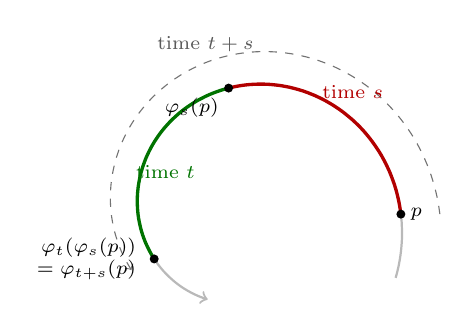
\begin{tikzpicture}[scale=0.9]
\draw[gray!55, thick, ->] plot[smooth] coordinates {(2.126,-0.899) (2.150,-0.810) (2.170,-0.721) (2.186,-0.632) (2.199,-0.543) (2.208,-0.453) (2.214,-0.364) (2.216,-0.275) (2.214,-0.187) (2.210,-0.098) (2.201,-0.011) (2.190,0.075) (2.175,0.161) (2.156,0.246) (2.135,0.329) (2.110,0.411) (2.082,0.492) (2.052,0.571) (2.018,0.648) (1.981,0.724) (1.942,0.798) (1.900,0.870) (1.855,0.940) (1.808,1.008) (1.758,1.073) (1.707,1.136) (1.653,1.197) (1.596,1.255) (1.538,1.311) (1.478,1.364) (1.417,1.415) (1.353,1.463) (1.288,1.508) (1.222,1.550) (1.154,1.590) (1.085,1.626) (1.015,1.660) (0.945,1.691) (0.873,1.719) (0.801,1.744) (0.728,1.765) (0.654,1.784) (0.581,1.800) (0.507,1.813) (0.433,1.823) (0.359,1.830) (0.285,1.834) (0.211,1.835) (0.138,1.833) (0.065,1.829) (-0.007,1.821) (-0.079,1.811) (-0.150,1.798) (-0.219,1.782) (-0.288,1.764) (-0.356,1.743) (-0.422,1.719) (-0.488,1.693) (-0.551,1.664) (-0.614,1.634) (-0.675,1.600) (-0.734,1.565) (-0.791,1.528) (-0.847,1.488) (-0.901,1.447) (-0.953,1.403) (-1.003,1.358) (-1.051,1.311) (-1.096,1.263) (-1.140,1.213) (-1.181,1.161) (-1.220,1.108) (-1.257,1.054) (-1.292,0.999) (-1.324,0.943) (-1.354,0.886) (-1.381,0.828) (-1.406,0.769) (-1.428,0.709) (-1.448,0.649) (-1.466,0.589) (-1.481,0.528) (-1.494,0.467) (-1.504,0.406) (-1.511,0.344) (-1.517,0.283) (-1.519,0.222) (-1.520,0.161) (-1.518,0.100) (-1.513,0.040) (-1.507,-0.020) (-1.497,-0.079) (-1.486,-0.137) (-1.473,-0.195) (-1.457,-0.252) (-1.439,-0.307) (-1.419,-0.362) (-1.397,-0.416) (-1.373,-0.469) (-1.347,-0.520) (-1.319,-0.570) (-1.289,-0.619) (-1.258,-0.666) (-1.225,-0.712) (-1.190,-0.756) (-1.154,-0.799) (-1.116,-0.840) (-1.077,-0.879) (-1.036,-0.916) (-0.995,-0.952) (-0.952,-0.986) (-0.908,-1.018) (-0.863,-1.048) (-0.817,-1.076) (-0.770,-1.102) (-0.723,-1.126) (-0.674,-1.149) (-0.626,-1.169) (-0.576,-1.187) (-0.526,-1.203)};
\draw[red!70!black, very thick] plot[smooth] coordinates {(2.200,0.000) (2.191,0.063) (2.181,0.126) (2.169,0.188) (2.155,0.250) (2.140,0.310) (2.123,0.371) (2.104,0.430) (2.083,0.489) (2.061,0.547) (2.038,0.604) (2.012,0.660) (1.986,0.715) (1.957,0.770) (1.928,0.823) (1.897,0.875) (1.864,0.926) (1.830,0.976) (1.795,1.025) (1.759,1.072) (1.721,1.119) (1.683,1.164) (1.643,1.208) (1.602,1.250) (1.560,1.291) (1.517,1.331) (1.472,1.369) (1.427,1.406) (1.382,1.442) (1.335,1.476) (1.287,1.509) (1.239,1.540) (1.190,1.569) (1.140,1.598) (1.090,1.624) (1.039,1.649) (0.988,1.673) (0.936,1.694) (0.884,1.715) (0.831,1.734) (0.778,1.751) (0.725,1.766) (0.671,1.780) (0.618,1.793) (0.564,1.803) (0.510,1.813) (0.456,1.820) (0.402,1.826) (0.348,1.831) (0.294,1.834) (0.240,1.835) (0.187,1.835) (0.133,1.833) (0.080,1.830) (0.027,1.825) (-0.025,1.819) (-0.077,1.811) (-0.129,1.802) (-0.180,1.791) (-0.231,1.779)};
\draw[green!45!black, very thick] plot[smooth] coordinates {(-0.231,1.779) (-0.287,1.764) (-0.343,1.747) (-0.397,1.728) (-0.451,1.708) (-0.504,1.686) (-0.555,1.663) (-0.606,1.637) (-0.656,1.611) (-0.705,1.583) (-0.753,1.553) (-0.799,1.522) (-0.845,1.490) (-0.889,1.456) (-0.931,1.422) (-0.973,1.385) (-1.013,1.348) (-1.052,1.310) (-1.089,1.270) (-1.125,1.230) (-1.160,1.188) (-1.193,1.146) (-1.224,1.103) (-1.254,1.059) (-1.283,1.014) (-1.310,0.968) (-1.335,0.922) (-1.359,0.875) (-1.381,0.828) (-1.402,0.780) (-1.420,0.731) (-1.438,0.683) (-1.453,0.634) (-1.467,0.584) (-1.480,0.535) (-1.490,0.485) (-1.499,0.435) (-1.507,0.385) (-1.512,0.335) (-1.517,0.285) (-1.519,0.235) (-1.520,0.185) (-1.519,0.136) (-1.517,0.086) (-1.513,0.037) (-1.508,-0.011) (-1.501,-0.060) (-1.492,-0.108) (-1.482,-0.155) (-1.471,-0.202) (-1.458,-0.248) (-1.444,-0.294) (-1.428,-0.339) (-1.411,-0.383) (-1.392,-0.427) (-1.372,-0.469) (-1.351,-0.511) (-1.329,-0.553) (-1.306,-0.593) (-1.281,-0.632)};
\draw[black!55, dashed, ->] plot[smooth] coordinates {(2.750,0.000) (2.732,0.125) (2.709,0.248) (2.680,0.369) (2.646,0.488) (2.607,0.604) (2.562,0.719) (2.513,0.830) (2.459,0.939) (2.401,1.044) (2.338,1.146) (2.271,1.244) (2.200,1.339) (2.125,1.430) (2.046,1.517) (1.964,1.600) (1.879,1.679) (1.791,1.753) (1.700,1.823) (1.606,1.888) (1.510,1.948) (1.412,2.004) (1.312,2.055) (1.211,2.101) (1.108,2.142) (1.003,2.179) (0.898,2.210) (0.792,2.236) (0.686,2.258) (0.579,2.274) (0.472,2.286) (0.366,2.292) (0.259,2.294) (0.154,2.291) (0.049,2.283) (-0.055,2.270) (-0.157,2.253) (-0.258,2.231) (-0.358,2.205) (-0.455,2.175) (-0.551,2.140) (-0.644,2.101) (-0.735,2.058) (-0.824,2.012) (-0.910,1.961) (-0.993,1.907) (-1.073,1.850) (-1.149,1.789) (-1.223,1.726) (-1.293,1.659) (-1.360,1.590) (-1.423,1.518) (-1.483,1.443) (-1.539,1.367) (-1.591,1.288) (-1.639,1.208) (-1.683,1.126) (-1.723,1.042) (-1.759,0.958) (-1.791,0.872) (-1.819,0.785) (-1.842,0.697) (-1.862,0.609) (-1.878,0.521) (-1.889,0.433) (-1.896,0.344) (-1.900,0.256) (-1.899,0.168) (-1.894,0.081) (-1.886,-0.005) (-1.873,-0.091) (-1.857,-0.175) (-1.837,-0.258) (-1.813,-0.339) (-1.786,-0.419) (-1.756,-0.498) (-1.722,-0.574) (-1.685,-0.648) (-1.644,-0.720) (-1.601,-0.790)};
\fill (2.200,0.000) circle (1.8pt) node[right, font=\scriptsize] {$p$};
\fill (-0.231,1.779) circle (1.8pt) node[below left, font=\scriptsize] {$\varphi_s(p)$};
\fill (-1.281,-0.632) circle (1.8pt) node[left=3pt, font=\scriptsize, align=right] {$\varphi_t(\varphi_s(p))$\\ $= \varphi_{t+s}(p)$};
\node[red!70!black, font=\scriptsize] at (1.520,1.730) {time $s$};
\node[green!45!black, font=\scriptsize] at (-1.123,0.601) {time $t$};
\node[black!65, font=\scriptsize] at (-0.558,2.393) {time $t + s$};
\end{tikzpicture}
